\documentclass[xcolor=dvipsnames, 9pt]{beamer}

\newenvironment{code}{\begin{semiverbatim} \begin{footnotesize}}
{\end{footnotesize}\end{semiverbatim}}

\usepackage{graphicx}
\usepackage{amssymb}
\usepackage{amsfonts}
\usepackage{amsmath}
\usepackage{hyperref}
\usepackage{natbib}
\usepackage{color}
\usepackage{pdfsync}
\usepackage{chancery}
\usepackage{movie15}
\usepackage{pgfpages}
\usepackage{fancyvrb}
\usepackage{colortbl}
\usepackage{multirow}

% \definecolor{white}{rgb}{255,255,255}
% \definecolor{darkred}{rgb}{0.5,0,0}
% \definecolor{darkgreen}{rgb}{0,0.5,0}
% \definecolor{lightblue}{rgb}{0,0,0.7}

% \hypersetup{colorlinks,
%   linkcolor=white,
%   filecolor=darkred,
%   urlcolor=lightblue,
%   citecolor=darkblue}

\usepackage{beamerthemesplit}
\usetheme{Copenhagen}
\usecolortheme[named=Violet]{structure} 
\setbeamertemplate{navigation symbols}{}
\setbeamertemplate{itemize items}[triangle]
\setbeamertemplate{enumerate items}[default]
%\setbeameroption{show notes on second screen}
% \logo{
\includegraphics[width = 2cm]{../images/logos/500px-NYU_logo.png}}

\newcommand{\R}{\mathbb{R}}
\renewcommand{\d}{\mathsf{d}}
\newcommand{\dd}{\partial}
\newcommand{\E}{\mathsf{E}}
\newcommand{\bb}{\mathbf}

\graphicspath{{../images/figures/}{../images/logos/}{../images/graphs}/}

\title{3 - Getting Started with NetworkX}
\author{Drew Conway and Aric Hagberg}
%\institute{
\includegraphics[width = 4cm]{500px-NYU_logo.png}}
\date{June 29, 2010}

\begin{document}
\begin{frame}[plain]
\titlepage
\end{frame}

\begin{frame}
\frametitle{Outline}
\begin{itemize}
\item Running Python and loading NetworkX
\item Finding what is in NetworkX
\item What is a NetworkX Graph (network)
\item Interacting with NetworkX graphs
\end{itemize}
\end{frame}

\begin{frame}
\frametitle{Running Python}
Running the interpreter (IPython)
Typing code at command line vs executing file
No GUI
\end{frame}


\begin{frame}[fragile]
\frametitle{Importing NetworkX}
Start Python

Import NetworkX using ``nx'' as a short name
\begin{block}{}
\begin{verbatim}
>>> import networkx as nx 
\end{verbatim}
\end{block}

\end{frame}

\begin{frame}
\frametitle{What's in Networkx?}
\begin{columns}[T]
\begin{column}{0.5\textwidth}
\centerline{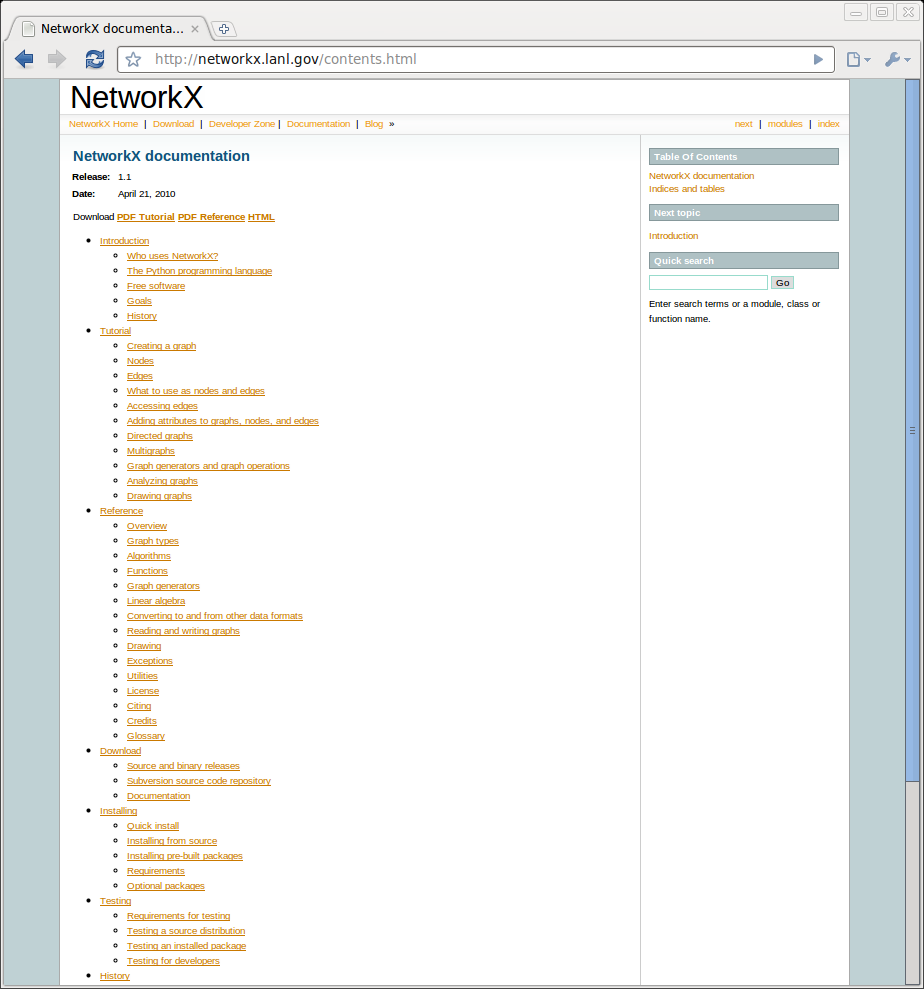
\includegraphics[width=1.0\columnwidth]{networkx-doc}}
\end{column}
\begin{column}{0.5\textwidth}
Figure showing command line help
\end{column}
\end{columns}
\end{frame}



\begin{frame}[fragile]
\frametitle{Adding nodes}

The basic $Graph$ class is used to hold the network information.
Nodes can be added as follows:
\begin{block}{}
\begin{verbatim}
>>> G=nx.Graph()
>>> G.add_node(1) # integer
>>> G.add_node('a') # string
>>> print G.nodes()
['a', 1]
\end{verbatim}
\end{block}

\end{frame}


\begin{frame}[fragile]
\frametitle{Feature: nodes can be ``anything''}

Nodes can be any hashable object such as strings,
numbers, files, functions, and more
\begin{block}{}
\begin{verbatim}
>>> import math
>>> G.add_node(math.cos) # cosine function
>>> fh=open('tmp.txt','w') 
>>> G.add_node(fh) # file handle
>>> print G.nodes()
[<built-in function cos>, 
<open file 'tmp.txt', mode 'w' at 0x30dc38>]
\end{verbatim}
\end{block}


\end{frame}


\begin{frame}[fragile]
\frametitle{Adding edges}
Edges, or links, between nodes are represented as tuples of nodes.  
They can be added simply
\begin{block}{}
\begin{verbatim}
>>> G.add_edge(1,'a')
>>> G.add_edge('b',math.cos)
>>> print G.edges()
[('b', <built-in function cos>), ('a', 1)]
\end{verbatim}
\end{block}

If the nodes do not already exist they are automatically added to the graph.

% FIXME add picture?


\end{frame}


\begin{frame}[fragile]
\frametitle{Edge can hold arbitrary data}

\begin{columns}[T]

\begin{column}{0.7\textwidth}
Any Python object is allowed as edge data 

(e.g. number, string, image, file, ip address)

Edge data assigned and stored in a Python dictionary (default empty).

\bigskip
Use Dijkstra's algorithm to find the shortest path:

\end{column}

\begin{column}{0.3\textwidth}
\centerline{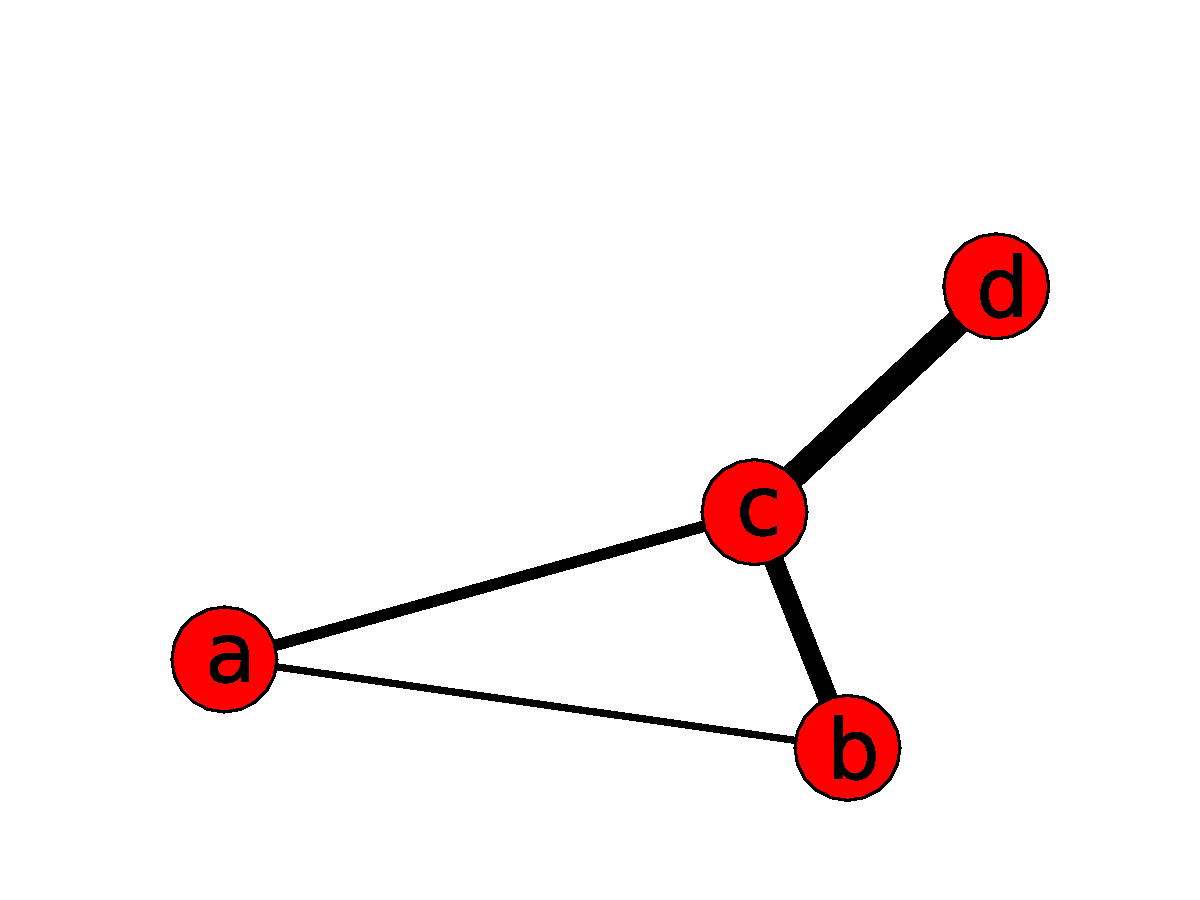
\includegraphics[width=1.5\columnwidth]{dijkstra}}
\end{column}
\end{columns}

\begin{block}{}
\begin{verbatim}
>>> G=nx.Graph()
>>> G.add_edge('a','b',weight=0.3)
>>> G.add_edge('b','c',weight=0.5)
>>> G.add_edge('a','c',weight=2.0)
>>> G.add_edge('c','d',weight=1.0)
>>> print nx.shortest_path(G,'a','d')
['a', 'c', 'd']
>>> print nx.shortest_path(G,'a','d',weighted=True)
['a', 'b', 'c', 'd']
\end{verbatim}
\end{block}

\end{frame}


% \begin{frame}[fragile]
% \frametitle{Inside NetworkX}

% It's ``Python all the way down''

% NetworkX uses a ``dictionary of dictionaries''

% Good for adjacency list representation (sparse graphs)

% \begin{itemize}
%   \item Node $n$ is a key in the $G.adj$ dictionary 
%   \item Data is a dictionary with neighbors as keys and data $1$
% \end{itemize}

% Representation of an undirected graph with the edges $A-B$, $B-C$
% \begin{block}{}
% \begin{verbatim}
% >>> G=nx.Graph()
% >>> G.add_edge('A','B')
% >>> G.add_edge('B','C')
% >>> print G.adj
% {'A': {'B': 1}, 
%  'B': {'A': 1, 'C': 1}, 
%  'C': {'B': 1}}
% \end{verbatim}
% \end{block}
% \end{frame}

% \begin{frame}[fragile]
% \frametitle{Dictionary of dictionaries}

% Guido van Rossum proposed a dictionary of lists 

% Allows the natural expressions (Eppstein)

% \begin{itemize}
%     \item ``{\tt n in G}'' to test if the graph $G$ contains node $n$ 
%     \item ``{\tt for n in G}'' to loop over all nodes
% \end{itemize}

% Advantages of ``dict of dict'' data structure
  
% \begin{itemize}
%   \item Find edges and remove edges with two dictionary look-ups 
%   \item Prefer to ``sets'' since data can be attached to edge
%     \begin{itemize}
%       \item $G[u][v]$ returns the edge object
%     \end{itemize}
% \end{itemize}

% \footnotesize

% \begin{itemize}
% \item
% Guido van Rossum.
% Python {P}atterns - {I}mplementing {G}raphs, 1998.
% \url{http://www.python.org/doc/essays/graphs/}

% \item
% David Eppstein.
% {PADS}, a library of {P}ython {A}lgorithms and {D}ata {S}tructures,
%   2008.
% \url{http://www.ics.uci.edu/\~eppstein/PADS/}
% \end{itemize}

% \end{frame}



\end{document}
